\documentclass{article}
\usepackage[left=3cm,right=3cm,top=2.5cm,bottom=2cm]{geometry} % page settings
\usepackage{amsmath} % provides many mathematical environments & tools
\usepackage{amssymb}
\usepackage{amsfonts}
\usepackage[spanish]{babel}
\usepackage[bookmarks]{hyperref}

\usepackage{multirow}
\usepackage{subfig}

\usepackage{algorithm}
\usepackage{algpseudocode}
\usepackage{pifont}

\usepackage[utf8]{inputenc}
\setlength{\parindent}{0mm}

\usepackage[parfill]{parskip}

% Para el código
\usepackage{listings}
\usepackage{xcolor}
\definecolor{gray}{rgb}{0.5,0.5,0.5}
\newcommand{\n}[1]{{\color{gray}#1}}
\lstset{numbers=left,numberstyle=\small\color{gray}}

% Entorno para estilo de ejercicios
\setlength{\parindent}{0pt}

\usepackage{color}   %May be necessary if you want to color links
\usepackage{hyperref}
\hypersetup{
    colorlinks=true, %set true if you want colored links
    linktoc=all,     %set to all if you want both sections and subsections linked
    linkcolor=blue,  %choose some color if you want links to stand out
}

\usepackage{graphicx}
\usepackage{subfig}

\usepackage{listings,textcomp}
\title{Problema del viajante de comercio\\ Travelling salesman problem}
\author{José Antonio Álvarez Ocete - Norberto Fernández de la Higuera \\ Javier Gálvez Obispo - Yábir García Benchakhtir }
\date{\today}

% Custom
\providecommand{\abs}[1]{\lvert#1\rvert}
\setlength\parindent{0pt}
\definecolor{Light}{gray}{.90}
\newcommand\ddfrac[2]{\frac{\displaystyle #1}{\displaystyle #2}}

% Listings
\lstset{literate=   % listings config
  {á}{{\'a}}1 {é}{{\'e}}1 {í}{{\'i}}1 {ó}{{\'o}}1 {ú}{{\'u}}1
  {Á}{{\'A}}1 {É}{{\'E}}1 {Í}{{\'I}}1 {Ó}{{\'O}}1 {Ú}{{\'U}}1
  {à}{{\`a}}1 {è}{{\`e}}1 {ì}{{\`i}}1 {ò}{{\`o}}1 {ù}{{\`u}}1
  {À}{{\`A}}1 {È}{{\'E}}1 {Ì}{{\`I}}1 {Ò}{{\`O}}1 {Ù}{{\`U}}1
  {ä}{{\"a}}1 {ë}{{\"e}}1 {ï}{{\"i}}1 {ö}{{\"o}}1 {ü}{{\"u}}1
  {Ä}{{\"A}}1 {Ë}{{\"E}}1 {Ï}{{\"I}}1 {Ö}{{\"O}}1 {Ü}{{\"U}}1
  {â}{{\^a}}1 {ê}{{\^e}}1 {î}{{\^i}}1 {ô}{{\^o}}1 {û}{{\^u}}1
  {Â}{{\^A}}1 {Ê}{{\^E}}1 {Î}{{\^I}}1 {Ô}{{\^O}}1 {Û}{{\^U}}1
  {œ}{{\oe}}1 {Œ}{{\OE}}1 {æ}{{\ae}}1 {Æ}{{\AE}}1 {ß}{{\ss}}1
  {ű}{{\H{u}}}1 {Ű}{{\H{U}}}1 {ő}{{\H{o}}}1 {Ő}{{\H{O}}}1
  {ç}{{\c c}}1 {Ç}{{\c C}}1 {ø}{{\o}}1 {å}{{\r a}}1 {Å}{{\r A}}1
  {€}{{\EUR}}1 {£}{{\pounds}}1 {ñ}{{\~{n}}}1
}

\lstset{    %listings config
	language=C++,
	belowcaptionskip=1\baselineskip,
	breaklines=true,
	frame=L,
	xleftmargin=0.1in,
	%otherkeywords={},
	showstringspaces=false,
	backgroundcolor=\color{white},
	basicstyle=\footnotesize\ttfamily,
	keywordstyle=\bfseries\color{purple!90!black},
	commentstyle=\itshape\color{gray!85!},
	identifierstyle=\color{blue!80!black},
	stringstyle=\color{green!60!black},
}

\begin{document}

\maketitle
\newpage
\tableofcontents
\newpage

\section{Descripción del problema}

En el problema del viajante de comercio (\textit{Travelling Salesman
  Problem}) se nos dan las coordenadas de un conjunto finito de
ciudades y se nos pide encontrar un recorrido de las misma de forma
que la distancia que recorramos sea la menor posible.

\section{Solucion ofrecidas}

En todas las soluciones descritas hemos usado una matriz de
adyaciencia, esto es, una matriz $M$ donde $m_{ij}$ nos indica la
distancia de la ciudad $i$ a la ciudad $j$. En nuestro caso se cumple
además que $m_{ji} = m_{ij}$ ya que consideramos que el camino que une
dos ciudades se puede recorrer en ambos sentidos.

\subsection{Solución branch and bound}

Branch and bound es una técnica similar a la de backtracking pero en
este caso la técnica de ramificación es distinta.

En lugar de desarrollar una rama del arbol hasta llegar a una hoja
desarrollando por niveles. Por tanto al mismo tiempo tenemos varios
nodos vivos. No los desarrollamos todos simultaneamente sino que los
desarrollamos en función de las expectativas que tenemos de cada nodo.

Cada nodo de nuestro grafo representa el estado parcial de una
solución y una cota que nos indica \textit{como de buena podría ser}
dicha solución. En cada iteración desarrollamos el nodo que siga
\textit{vivo} y que mejor cota tenga.


\begin{algorithm}[H]
\caption{Algoritmo Branch and Bound}
\begin{algorithmic}
\State solution = next PriorityQueue($<$length, path$>$)
\If {path is completed}
\State localLength = path.length
\Else
\State minPossible = estimate path
\State localLength = solution.length
\EndIf
\If {localLength $<$ best Solution}
\For {city not in path} 
\State add city to the path
\State compute new min Length
\State Explore new solution if it's worth
\EndFor
\EndIf
\end{algorithmic}
\end{algorithm}

Como función que nos permite estimar lo buena que puede llegar a ser
una solución calculamos la suma de los mínimos de cada fila en la
matriz de adyaciencia que no haya sido ya visitada (no se encuentra en
el camino actual).

\begin{lstlisting}
  double estimacion(vector<int> &candidates, vector<vector<double> > &cities){

    double result = 0;
    double row_min;

    for(int i = 0; i < cities.size()-1; i++){
      if(!visitado(i,candidates)){
        result += rowMin(i, cities[i]);
      }
    }

    return result;

  }
\end{lstlisting}

Además para mejorar la eficiencia de nuestro algoritmo hemos partido
de una solución inicial que podemos considerar \textit{buena}, es
decir, próxima a la solución óptima en cuanto a distancia del
recorrido se refiere. De esta manera conseguimos que nuestro algoritmo
explore menos nodos (realice más podas) y por lo tanto estamos
mejorando su eficiencia empírica.

La solución inicial que nos ha permitidos podar la hemos basado en el
algoritmo genético que desarrollamos en la práctica anterior y que de
manera rápida nos ofrecía una solución bastante buena. De esta manera
a la hora de realizar poda podíamos descartar más resultados de manera
eficiente.

Para decidir la ciudad de inicio para el recorrido empleamos la siguiente función:

\begin{lstlisting}
  int farthest(vector<pair<double, double> > &coordinates){
    pair<double,double> centro(0,0);
    double dist, max = 0;
    int mejor = 0;

    for(int i = 0; i < coordinates.size(); i++){
      centro.first += coordinates[i].first;
      centro.second += coordinates[i].second;
    }
    
    centro.first /= coordinates.size();
    centro.second /= coordinates.size();
    
    for(int i = 0; i < coordinates.size(); i++){
      dist = distance(coordinates[i], centro);
      if(dist > max){
     	max = dist;
     	mejor = i;
      }
    }

    return mejor;
  }
\end{lstlisting}

Con esto conseguimos que nuestra primera ciudad sea la que está mas
lejos del centro y en nuestro recorrido nos vamos acercando al
centro. Esta técnica es una de las que se propuso en ocasiones
anteriores y que hemos considerado buena idea aplicar.

\subsection{Solución usando backtracking}

En la solución propuesta de backtracking realizamos una exploración
vertical del arbol de soluciones. Nuestro nodo en desarrollo sera el
primer hijo que podamos explorar hasta llegar a un nodo terminal y una
vez ahí pasará a ser nodo muerto.

Una posible implementación de dicho algoritmo sería la siguiente:

\begin{lstlisting}
  
void backtracking(int pos, pair<double, vector<int> > sol, vector<vector<double> > &cities, pair<double, vector<int> > &best){
  if(pos < cities.size()){
    for(int i = 1; i < cities.size(); i++){
  		if(!visitado(i, sol.second)){
  			sol.second[pos] = i;
        sol.first = compute_length(sol.second, cities);
  			if(sol.first < best.first)
          backtracking(pos + 1, sol, cities, best);
    	}
    }
  } else if(best.first < best.first)
    best = sol;
}

\end{lstlisting}

Inicialmente y sin estudiar empíricamente los algoritmos vemos que
ambos tienen una eficiencia teórica de $O(n!)$ ya que estamos
estudiando todas las combinaciones posibles de ordenar un conjunto de
$n$ candidatos. Sin embargo cabría esperar que no se comportasen de
esta manera ya que por ejemplo en el algoritmo de branch and bound no
estamos desarrollando todos los nodos por lo que el cardinal de nodos
que tenemos que trazar es mucho menos del total que podríamos
recorrer. En el algoritmo de backtracking usamos una técnica similar
que nos permite eliminar soluciones sin tener que explorar la rama al
completo.

\section{Análisis empírico de los algoritmos}

Para estudiar la eficiencia empírica de los resultados se ha utilizado
un ordenador con las siguiente caracterísiticas:

\begin{itemize}
\item CPU: Intel Pentium G3258 (2) @ 3.200GHz
\item Memoria RAM: 7876MiB
\item Kernel: 4.13.0-36-generic
\item OS: Linux Mint 18.3 Sylvia x86\_64
\end{itemize}

Debido a la complejidad del algoritmo no fuimos capaces de obtener
resultados para mapas muy grandes y en particular para los mapas
ofrecidos salvo para el caso de \textit{ulysses16}. Es por esto que se
ha procedido a la creación de mapas propios, los cuales se acompañan a
este documento y en los que sí hemos podido probar nuestro algoritmo.

\begin{table}[H]
\centering
\caption{Comparativa de longitud y tiempo (seg) para cada algoritmo}
\label{my-label}
\begin{tabular}{lll}
\hline
\multicolumn{1}{|l|}{Longitud} & \multicolumn{1}{l|}{Branch and bound} & \multicolumn{1}{l|}{Backtracking} \\ \hline
\multicolumn{1}{|l|}{19.9247}  & \multicolumn{1}{l|}{3E-06}            & \multicolumn{1}{l|}{2E-06}        \\ \hline
\multicolumn{1}{|l|}{51.6735}  & \multicolumn{1}{l|}{6E-06}            & \multicolumn{1}{l|}{3E-06}        \\ \hline
\multicolumn{1}{|l|}{59.4593}  & \multicolumn{1}{l|}{1.7E-05}          & \multicolumn{1}{l|}{5E-06}        \\ \hline
\multicolumn{1}{|l|}{56.4986}  & \multicolumn{1}{l|}{5E-05}            & \multicolumn{1}{l|}{1.6E-05}      \\ \hline
\multicolumn{1}{|l|}{119.193}  & \multicolumn{1}{l|}{0.000148}         & \multicolumn{1}{l|}{6.2E-05}      \\ \hline
\multicolumn{1}{|l|}{150.371}  & \multicolumn{1}{l|}{0.000919}         & \multicolumn{1}{l|}{0.000281}     \\ \hline
\multicolumn{1}{|l|}{255.254}  & \multicolumn{1}{l|}{0.001052}         & \multicolumn{1}{l|}{0.000763}     \\ \hline
\multicolumn{1}{|l|}{361.223}  & \multicolumn{1}{l|}{0.003113}         & \multicolumn{1}{l|}{0.003867}     \\ \hline
\multicolumn{1}{|l|}{464.618}  & \multicolumn{1}{l|}{0.015933}         & \multicolumn{1}{l|}{0.021076}     \\ \hline
\multicolumn{1}{|l|}{476.531}  & \multicolumn{1}{l|}{0.014079}         & \multicolumn{1}{l|}{0.049719}     \\ \hline
\multicolumn{1}{|l|}{586.246}  & \multicolumn{1}{l|}{0.193942}         & \multicolumn{1}{l|}{3.49537}      \\ \hline
\multicolumn{1}{|l|}{755.058}  & \multicolumn{1}{l|}{0.046548}         & \multicolumn{1}{l|}{0.676337}     \\ \hline
\multicolumn{1}{|l|}{1040.99}  & \multicolumn{1}{l|}{0.234971}         & \multicolumn{1}{l|}{9.97742}      \\ \hline
\multicolumn{1}{|l|}{1146.6}   & \multicolumn{1}{l|}{0.311181}         & \multicolumn{1}{l|}{29.1998}      \\ \hline
                               &                                       &                                  
\end{tabular}
\end{table}


Para visualizar los datos los hemos representado en una gráfica de
línieas donde comparamos ambos algoritmos:

\begin{figure}[H]
  \centering
  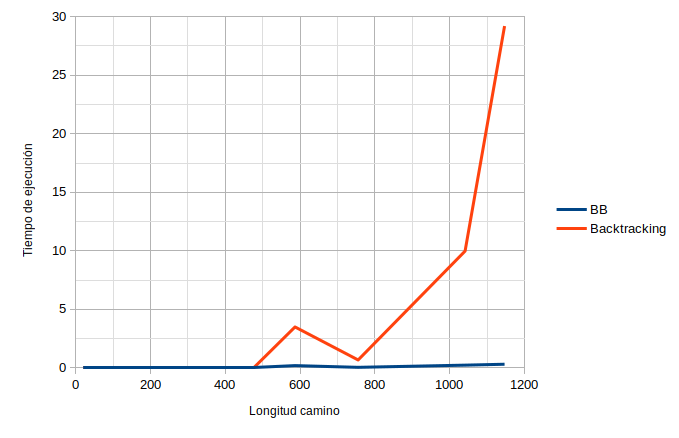
\includegraphics[width=0.8\textwidth]{comparativa.png}
  \caption{Comparativa de los algoritmos de backtracking y branch and bound}
\end{figure}


\section{Comparativa con los algoritmos greedy}

Si comparamos por ejemplo con el algoritmo greedy
\textit{cheapInserction} obtenemos los resultados siguientes:

\begin{table}[H]
\centering
\caption{Resultados para un algoritmo greedy}
\label{my-label}
\begin{tabular}{|l|l|}
\hline
19.9247 & 4E-06 \\ \hline
51.6735 & 2E-06 \\ \hline
59.4593 & 1E-06 \\ \hline
62.8659 & 2E-06 \\ \hline
123.26  & 2E-06 \\ \hline
150.371 & 3E-06 \\ \hline
300.216 & 3E-06 \\ \hline
361.223 & 3E-06 \\ \hline
494.908 & 2E-06 \\ \hline
476.531 & 4E-06 \\ \hline
794.865 & 4E-06 \\ \hline
581.918 & 4E-06 \\ \hline
1005.65 & 5E-06 \\ \hline
1070.15 & 5E-06 \\ \hline
1272.67 & 6E-06 \\ \hline
\end{tabular}
\end{table}

En esta tabla podemos contrastar de manera clara como en tiempo los
algoritmos greedy ganan a los de branch and bound pero los recorridos
que obtienen no son mejores. A continuación se han representado uno de
los resultados que se obtienen con branch and bound y usando
algoritmos greedy.

\begin{figure}[H]
  \centering
  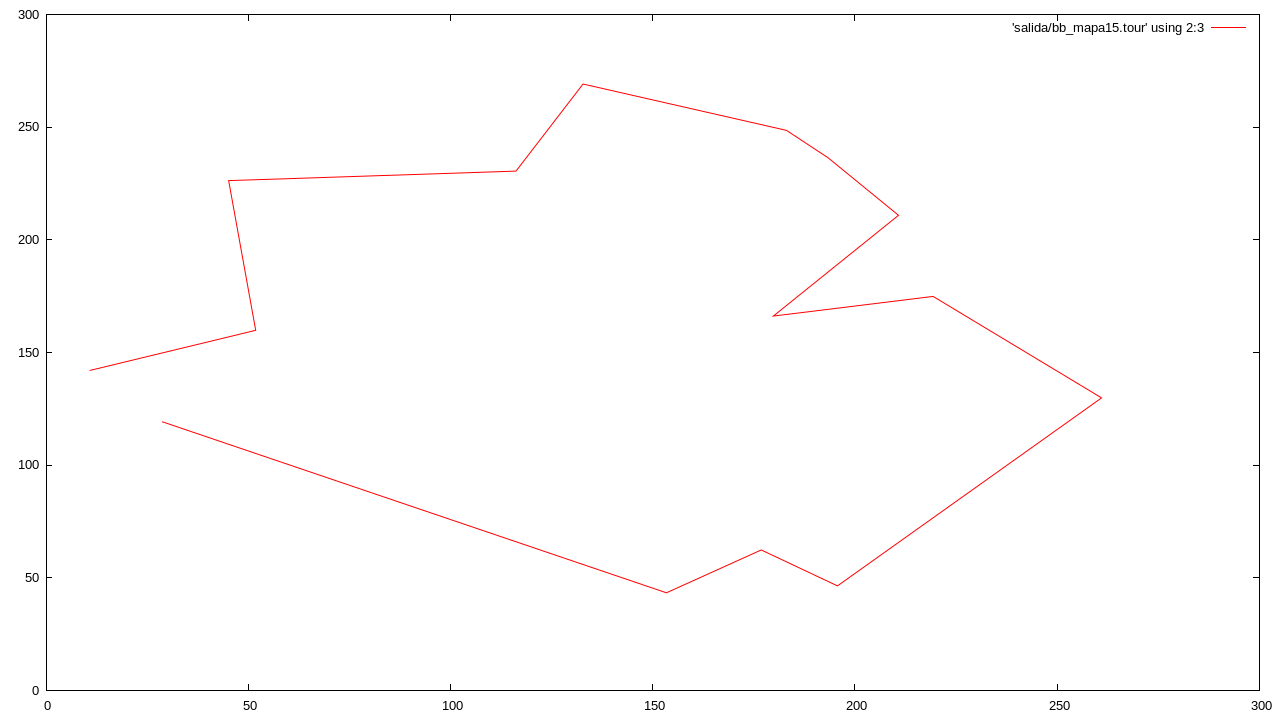
\includegraphics[width=0.8\textwidth]{bb_mapa15}
  \caption{Algoritmo de branch and bound}
\end{figure}

\begin{figure}[H]
  \centering
  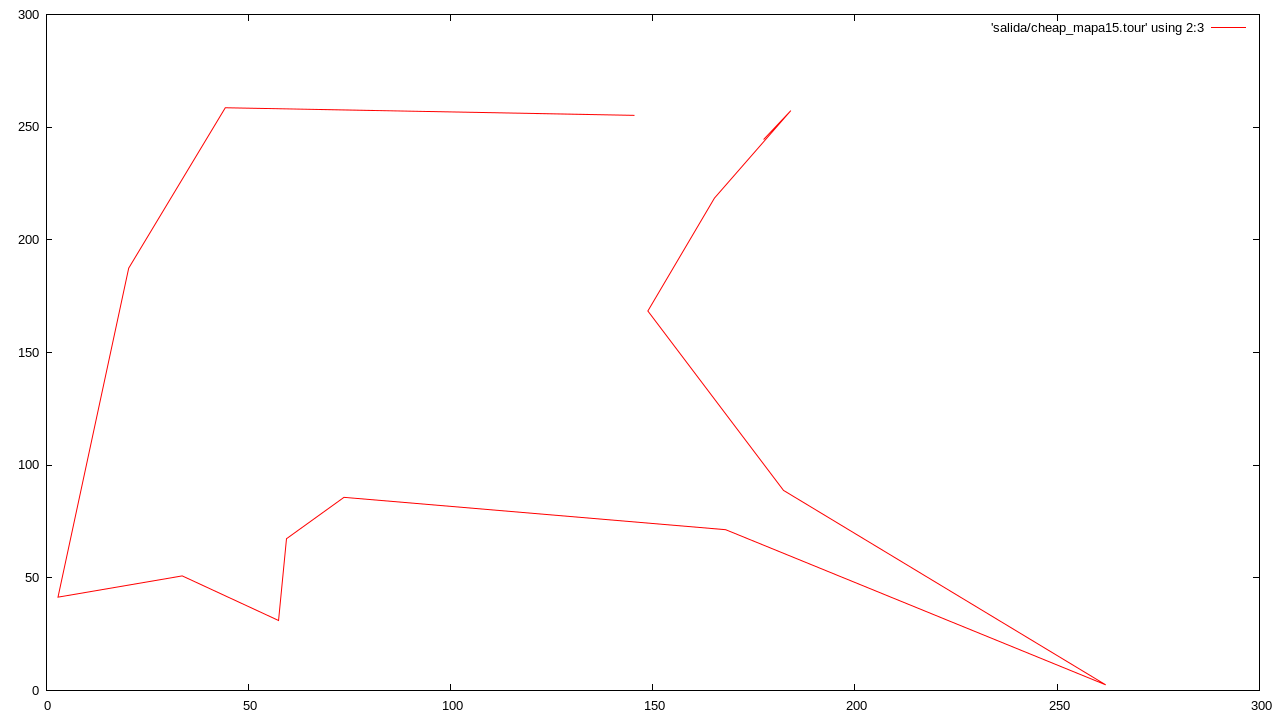
\includegraphics[width=0.8\textwidth]{cheap_mapa15}
  \caption{Algoritmo greedy}
\end{figure}



\section{Conclusiones}

En este estudio hemos podido comprobar como la técnica de branch and
bound ofrece resultados en tiempo mejores que la de backtracking. Pese
a que ambos devuelven la mejor solución siempre debido a que en ambos
algoritmos estamos explorarndo todo el grafo de soluciones posibles.

En segundo lugar los resultados demuestran que la técnica de branch
and bound obtiene mejores tiempos de ejecución para encontrar la misma
solución que empleando la técnica de backtracking.

Estos resultados son los que cabría esperar de este tipo de algoritmos
donde se prima lo buena que sea la solución más que el tiempo que
tarde en obtenerse.


\end{document}
